\section{Sprint 4: Generador de proyectos Django}
\label{sec:generador-proytectos}

Tras la implementación del LLM y el sistema de schema funcionando correctamente, el siguiente paso era el más complejo del proyecto, ya que requería 
coordinar múltiples llamadas al LLM de forma secuencial garantizando 
que cada fichero generado fuese compatible con los anteriores. Dicho paso era convertir el schema aprobado por el usuario en un proyecto Django completo, funcional y desplegable. Durante este sprint del proyecto surgió el fichero más importante hasta la fecha: \textbf{utils/generator/project\_generator}, el núcleo de WebBuilder.


\subsection{Arquitectura del generador}
\label{subsec:arquitectura-generador}

El generador se organiza como un orquestador de siete pasos secuenciales, cada uno con su responsabilidad concreta y encargado de producir uno o varios ficheros del proyecto final.
El LLM interviene en los primeros seis pasos, que se encargan de la creación de ficheros, pero en el séptimo paso ya no interviene, y se concluye la ejecución con el ensamblaje de todos los ficheros generados anteriormente.

\begin{itemize}
    \item \textbf{Paso 1 — Estructura de páginas}: decide qué páginas 
    tendrá el sitio, sus URLs, sus nombres de vista y si cada página es 
    un listado, una página de detalle o una portada. El resultado guiará 
    todos los pasos siguientes.
    
    \item \textbf{Paso 2 — models.py}: genera el modelo de datos Django 
    adaptado a los campos del dataset.
    
    \item \textbf{Paso 3 — views.py y urls.py}: genera las vistas para 
    cada página del paso 1. El fichero \texttt{urls.py} se construye en 
    Python directamente a partir de la lista de páginas, sin intervención 
    del modelo.
    
    \item \textbf{Paso 4 — base.html}: genera la plantilla base con la 
    estructura HTML común: cabecera, navegación y bloque de contenido.
    
    \item \textbf{Paso 5 — Templates por página}: genera un template HTML 
    independiente para cada página, adaptado a su tipo y a los campos del 
    dataset.
    
    \item \textbf{Paso 6 — load\_data.py}: genera un comando de gestión 
    Django que descarga los datos de la API original y los inserta en la 
    base de datos del sitio generado, garantizando contenido real desde 
    el primer arranque.
    
    \item \textbf{Paso 7 — Archivos fijos}: se ensamblan los ficheros de 
    infraestructura independientes del dataset: \texttt{settings.py}, 
    \texttt{manage.py}, \texttt{wsgi.py}, \texttt{requirements.txt}, 
    \texttt{Dockerfile} y \texttt{entrypoint.sh}.
\end{itemize}


Como ejemplo representativo, se muestra el prompt que se envía 
al LLM en el Paso 2 para la generación del fichero \texttt{models.py}. 
A diferencia de prompts más abiertos, este es restrictivo, la causa es que el código generado debe ser sintácticamente correcto sin ninguna intervención humana, por lo que cada regla busca eliminar un tipo 
de error concreto observado durante las pruebas.

\begin{lstlisting}[caption={Prompt de sistema para la generación de models.py}, 
label={lst:models-system}]
Eres un desarrollador Django experto en Python y Tailwind CSS.
REGLA ABSOLUTA: devuelves ÚNICAMENTE código puro, sin ningún tipo de 
Markdown. Sin ```, sin ```python, sin explicaciones. Solo el código.
\end{lstlisting}

\begin{lstlisting}[caption={Prompt de usuario para la generación de models.py}, 
label={lst:models-user}]
SITIO: <nombre del sitio>

CAMPOS:
[{"key": "campo1", "label": "Etiqueta 1"}, ...]

ROLES SEMÁNTICOS INFERIDOS (clave: rol):
  - campo1: title
  - campo2: numeric
  - campo3: image

DATOS DE EJEMPLO:
[{"campo1": "valor1", "campo2": 42, ...}, ...]

REGLAS:
- CRÍTICO: tu respuesta debe empezar EXACTAMENTE con
  'from django.db import models'. Sin nada antes.
- Un modelo llamado 'Item' con los campos del schema.
- rol 'numeric'   -> FloatField(null=True, blank=True)
- rol 'image'     -> URLField(max_length=500, blank=True)
- rol 'date'      -> DateField(null=True, blank=True)
- rol 'boolean'   -> BooleanField(null=True, blank=True)
- rol 'long_text' -> TextField(blank=True)
- rol 'title'     -> CharField(max_length=300, blank=True)
- rol 'text'      -> CharField(max_length=500, blank=True)
- Todos los campos opcionales (blank=True / null=True).
- Añade created_at = models.DateTimeField(auto_now_add=True).
- __str__ devuelve el campo más representativo.
- NUNCA uses JSONField ni CharField para listas.

\end{lstlisting}

El resultado final es un diccionario Python donde cada clave es una ruta relativa de fichero y cada valor es su contenido. Este diccionario se guarda en el campo \texttt{project\_files} del modelo \texttt{GeneratedSite}, comentado más adelante en la subsección~\ref{subsec:modelo-generatedsite}

A modo de ejemplo, la Figura~\ref{fig:Primera-generación} muestra el resultado de una 
de las primeras generaciones reales del sistema, utilizando la API pública 
\texttt{fakestoreapi.com/products}, que devuelve un catálogo de productos 
con campos como título, precio, categoría e imagen. El sitio generado, aunque 
funcional, refleja las limitaciones del generador: 
diseño genérico, campos mostrados en crudo, sin estilos visuales y sin las imágenes de la base de datos.

\begin{figure}[H]
    \centering
    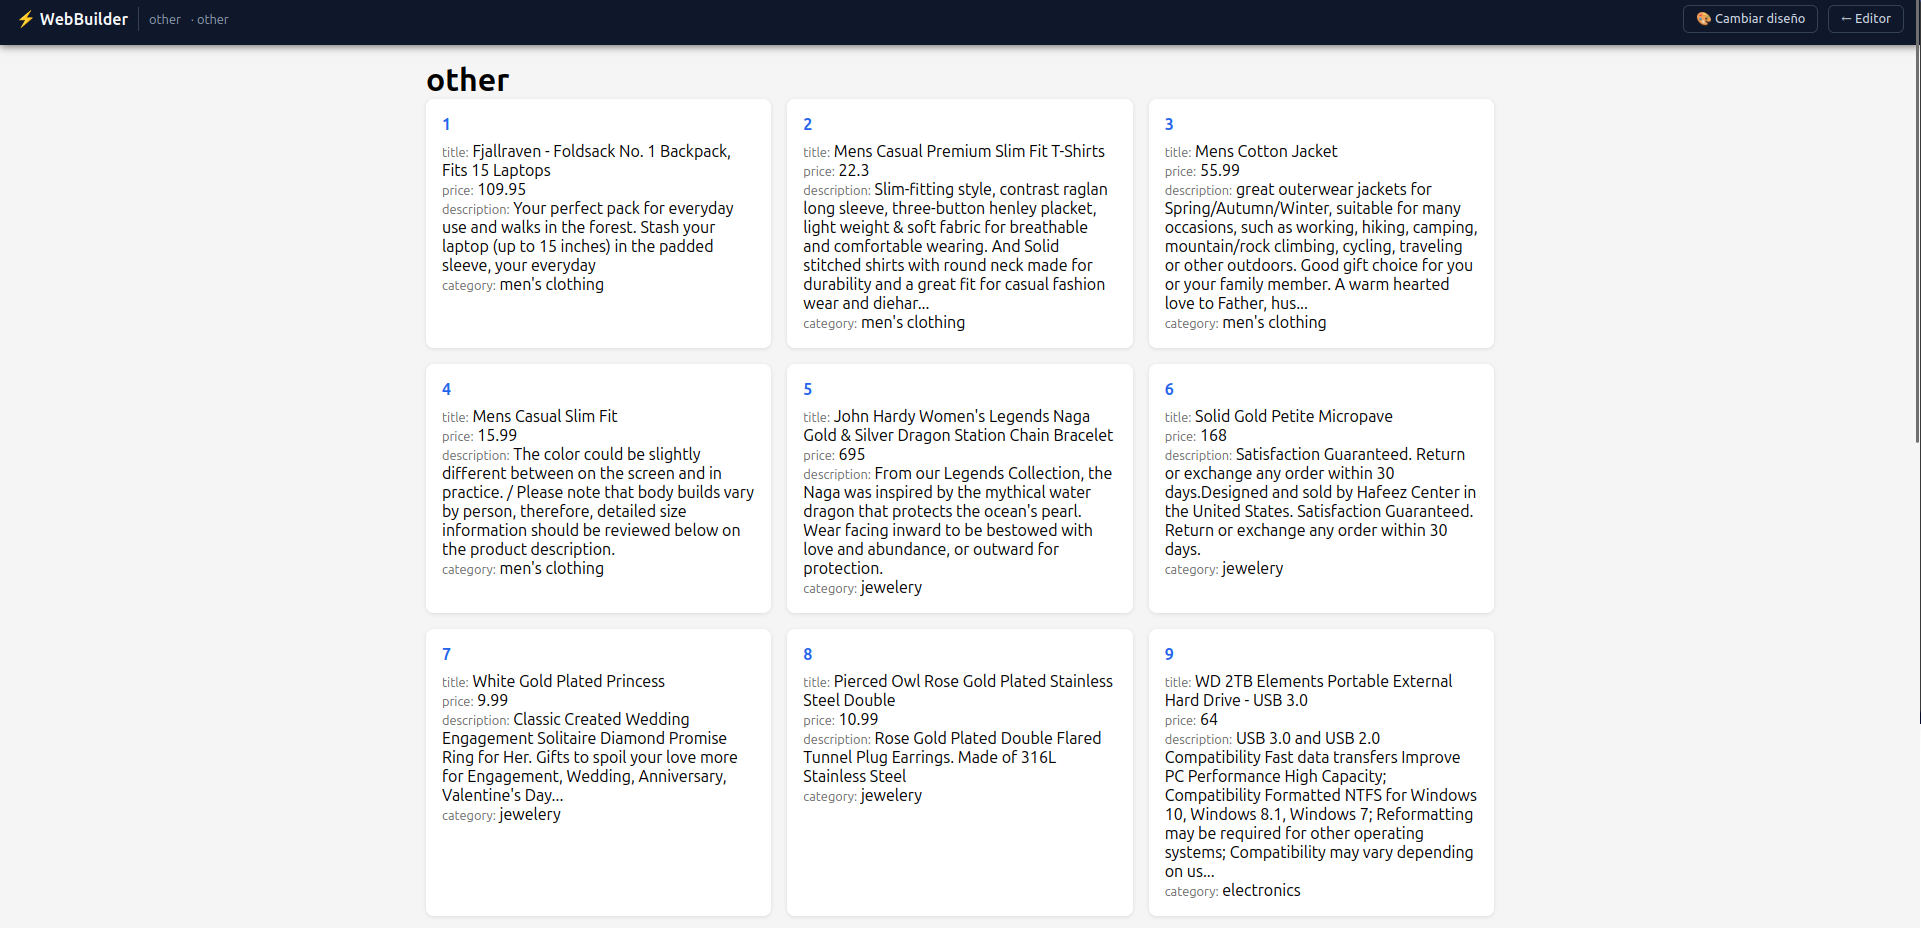
\includegraphics[width=\textwidth]{img/oldversions/firstgenPRODUCTS}
    \caption{Primera web generada por WebBuilder a partir de la API FakeStore}
    \label{fig:Primera-generación}
\end{figure}

En la Figura~\ref{fig:generador-7-pasos} se muestra la secuencia completa de los siete pasos del generador.

\begin{figure}[H]
    \centering
    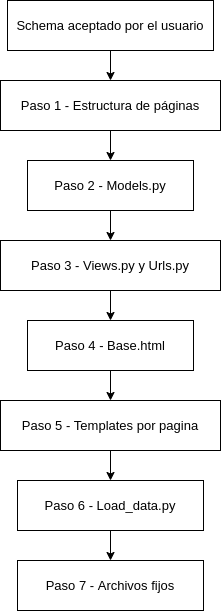
\includegraphics[width=0.3\textwidth]{img/disenoimplementacion/pasosgeneradorfase4.png}
    \caption{Los 7 pasos del generador de proyectos Django}
    \label{fig:generador-7-pasos}
\end{figure}

\subsection{Fallbacks de generación}
\label{subsec:fallbacks-generacion}

Durante las pruebas de generación se comprobó que las alucinaciones del LLM 
eran constantes y que pulir cada prompt requeriría un trabajo considerable. 
El LLM cometía fallos en cualquiera de los pasos, devolviendo código vacío, 
con errores de sintaxis o código no adaptado al paso correspondiente. Para 
garantizar que el proyecto resultante fuese siempre desplegable, se añadió 
un fallback por cada paso del generador.

El funcionamiento era el siguiente: si la respuesta del LLM era vacía o 
inválida, el sistema activaba automáticamente una versión mínima pero 
funcional del fichero en cuestión. Por ejemplo, el fallback de 
\textbf{models.py} generaba un modelo genérico llamado \texttt{Item} con 
un campo \texttt{CharField} por cada campo del dataset. El fallback de 
\textbf{views.py} generaba vistas básicas de listado y detalle sobre ese 
mismo modelo. El fallback de \textbf{pages} definía tres páginas fijas: 
portada, catálogo y detalle. Y el fallback de \textbf{load\_data.py} 
generaba un comando mínimo de carga de datos a partir de la URL original 
de la API.

De esta forma, aunque el LLM produjese un resultado de baja calidad en 
algún paso, el proyecto generado siempre sería desplegable, aunque con 
una interfaz más genérica.

\subsection{Evolución del modelo de datos}
\label{subsec:modelo-generatedsite}

El modelo \texttt{GeneratedSite} fue variando durante este sprint para reflejar 
los nuevos estados del sistema. Se añadieron los campos \texttt{project\_files} 
para almacenar todos los ficheros generados, \texttt{project\_name} con el nombre 
del proyecto y \texttt{preview\_url} para guardar la URL del sitio desplegado 
(explicado en la subsección~\ref{subsec:workflow-despliegue}). Además se 
incorporaron dos nuevos campos de estado cuya evolución se muestra en la 
Tabla~\ref{tab:estados-generatedsite}.

\begin{table}[H]
    \centering
    \begin{tabular}{|l|l|p{7cm}|}
        \hline
        \textbf{Campo} & \textbf{Valores} & \textbf{Significado} \\
        \hline
        \textbf{generation\_status} & pending & El sitio está en espera de ser generado \\
        \hline
        & generating & El generador está produciendo los ficheros \\
        \hline
        & ready & Los ficheros han sido generados correctamente \\
        \hline
        & error & La generación ha fallado en algún paso \\
        \hline
        \textbf{deploy\_status} & idle & El contenedor no ha sido desplegado aún \\
        \hline
        & deploying & El workflow de n8n está construyendo la imagen \\
        \hline
        & done & El contenedor está en funcionamiento \\
        \hline
        & error & El despliegue ha fallado en algún paso \\
        \hline
    \end{tabular}
    \caption{Estados del modelo GeneratedSite en el sprint 4}
    \label{tab:estados-generatedsite}
\end{table}

Esta separación entre el estado de generación y el estado de despliegue 
permitía saber con precisión en qué punto del proceso se encontraba cada sitio.

\subsection{Dockerfile, entrypoint y requirements}
\label{subsec:dockerfile}

Cada proyecto generado incluía un \texttt{Dockerfile}, un script \texttt{entrypoint.sh} y un fichero \texttt{requirements.txt} que en conjunto automatizaban completamente el arranque del sitio. El objetivo era que cualquier proyecto generado por WebBuilder se desplegase mediante Docker pulsando un botón, sin configuración manual por parte del usuario.

El \texttt{Dockerfile} partía de la imagen oficial \texttt{python:3.12}. Copiaba el \\ \texttt{requirements.txt}, instalaba las dependencias con \texttt{pip} y copiaba el resto del proyecto. Hasta entonces el puerto expuesto era el 8000, sobre el que se serviría la aplicación, esto variaría más adelante con la mejora del flujo de despliegue de n8n.

El fichero \texttt{requirements.txt} incluido en cada proyecto generado contenía únicamente las dependencias mínimas para el funcionamiento del sitio: \texttt{django>=4.2,<6.0} como framework web, \texttt{requests>=2.28} para que el comando \texttt{load\_data} pudiera descargar los datos de la API original, y \texttt{gunicorn>=21.0} como servidor de producción. La decisión de mantener las dependencias al mínimo fue intencionada: cuantas menos dependencias tenga el proyecto generado, menos probabilidades hay de que el \texttt{docker build} falle por incompatibilidades o paquetes no disponibles.

El script \texttt{entrypoint.sh} era el responsable del arranque completo del sitio, los pasos que ejecutaba eran los siguientes:

\begin{enumerate}
    \item \textbf{Generación de migraciones}: ejecutaba \texttt{python manage.py makemigrations siteapp} para crear los ficheros de migración a partir del \texttt{models.py}, siendo \texttt{siteapp} el nombre de la aplicación interna del proyecto generado. Este paso quedó obsoleto tras el desarrollo del módulo \texttt{migrations\_generator.py}, descrito en la Sección~\ref{subsec:refactor-generador-modulos}, encargado de parsear el \texttt{models.py} generado por el LLM y construir el fichero \\ \texttt{0001\_initial.py} directamente, incluyéndolo ya en el ZIP antes del despliegue. De este modo, cuando el contenedor arranca y el \texttt{entrypoint.sh} ejecuta \texttt{makemigrations}, el fichero ya existe y Django simplemente lo detecta sin generar nada nuevo.
    \item \textbf{Aplicación de migraciones}: ejecutaba \texttt{python manage.py migrate} para crear las tablas en la base de datos SQLite del contenedor.
    \item \textbf{Carga de datos}: ejecutaba \texttt{python manage.py load\_data}, el comando generado por el LLM en el paso 6 del generador, que descargaba los datos de la API original e insertaba los registros en la base de datos.
    \item \textbf{Arranque del servidor}: lanzaba Gunicorn con dos workers (capacidad para atender 2 peticiones simultáneas) y un timeout de 120 segundos para servir la aplicación Django en el puerto 8000.
\end{enumerate}

Esta secuencia garantizaba que al acceder al sitio por primera vez ya estuviera completamente funcional: base de datos creada, datos cargados y servidor en marcha. El uso de 
Gunicorn en lugar del servidor de desarrollo de Django era una decisión deliberada para que los sitios generados tuvieran un nivel mínimo de robustez en producción.


\subsection{Workflow de despliegue n8n}
\label{subsec:workflow-despliegue}

En paralelo al desarrollo del generador de archivos, se fue construyendo el workflow más importante del proyecto, encargado del despliegue de las páginas.

La decisión de delegar el despliegue en n8n y no en Django respondía 
a un problema técnico concreto: el proceso de build de Docker puede 
tardar varios minutos, y ejecutarlo de forma síncrona desde Django 
bloquearía el servidor durante ese tiempo. Al separarlo y crearlo con n8n, Django lo único que tiene que hacer es el enviar la señal para que comience la ejecución del workflow.

Esta señal se envía desde la ruta \texttt{/webhook/webbuilder-deploy}. Django realiza una llamada POST con el nombre del proyecto como parámetro y a partir de aquí el workflow se ejecuta siguiendo los siguientes nodos sucesivamente:

\begin{enumerate}
    \item \textbf{Descomprimir ZIP}: el primer nodo crea el directorio de despliegue en \\ \texttt{/files/deploys/<project\_name>} y descomprime el ZIP del proyecto generado en un subdirectorio \texttt{src/}.
    \item \textbf{Restablecer contenedor}: antes de construir la nueva imagen, el workflow intenta detener y eliminar cualquier contenedor anterior con el mismo nombre (\texttt{wb\_<project\_name>}). Si el contenedor no existe, el error se ignora y el flujo continúa sin interrupciones.
    
    \item \textbf{Elegir puerto}: el nodo escanea los puertos actualmente en uso por Docker en el rango 8100--8999 y selecciona el primer puerto libre disponible. Si no hay ningún puerto libre en ese rango, el flujo lanza un error controlado.
    
    \item \textbf{Docker Build}: ejecuta \texttt{docker build} sobre el directorio del proyecto con un timeout de 5 minutos. Si el build falla, captura los últimos 500 caracteres de los logs de error para facilitar el diagnóstico.
    
    \item \textbf{Docker Run}: arranca el contenedor en modo \emph{detached} con el nombre y el puerto asignados, mapeando el puerto elegido al puerto interno 8000 del contenedor.
    
    \item \textbf{Verificar Docker}: espera 20 segundos para dar tiempo al \texttt{entrypoint.sh} a ejecutar las migraciones y cargar los datos, y luego comprueba que el contenedor sigue en funcionamiento. Si el contenedor ha caído, recupera las últimos 40 líneas de sus logs y lanza un error con esa información para facilitar el diagnóstico.

    \item \textbf{Responder al webhook}: si todo ha ido bien, devuelve a Django un JSON con la URL del preview, el nombre del contenedor y el puerto asignado, que WebBuilder almacena en el campo \texttt{preview\_url} del modelo \texttt{GeneratedSite}.
\end{enumerate}

Este diseño garantiza que el usuario siempre recibe una respuesta clara: si el despliegue tiene éxito obtiene la URL del sitio generado, y si falla en cualquier paso Django es notificado con información suficiente para actualizar el estado del sitio a \texttt{error} y mostrar un mensaje al usuario explicando lo ocurrido.

En la Figura~\ref{fig:workflow-despliegue} se muestra el flujo completo del workflow de despliegue.

\begin{figure}[H]
    \centering
    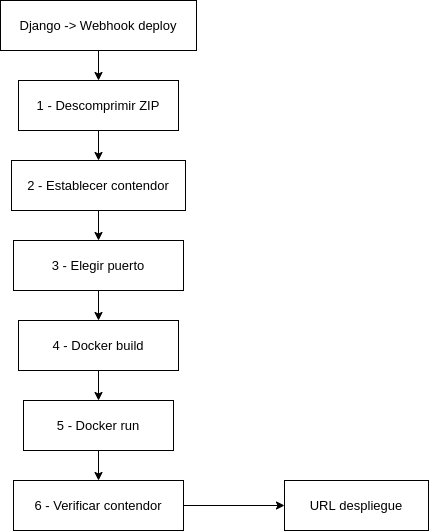
\includegraphics[width=0.5\textwidth]{img/disenoimplementacion/workflowdespliegue.png}
    \caption{Workflow de despliegue n8n}
    \label{fig:workflow-despliegue}
\end{figure}